\clearpage
\section{Coursework 1 (Part 2): \\ A Homing Robot}

In this part of the coursework we get to grips with some slightly more 
difficult
programming tasks, consider the problem of ensuring that software is working
correctly, and experiment with additional elements of the Java language. \\

\noindent
The main aim of the exercises in this chapter is to guide you through building
a robot controller which will make the robot home in on the target. The robot 
controllers which we have built so far will ensure that the robot eventually
reaches the target; however, they will not direct the robot in any 
meaningful way. The
target is reached because the robot chooses directions randomly and if 
enough random moves are made then the robot will eventually find the target.
The trouble with this method is that it may take a long time for the 
robot to reach the target, particularly if the maze is very large. \\

\noindent
If the robot controller is able to sense where the target is located, then
a better search technique can be applied. Rather than the robot moving 
randomly, it could attempt to move closer to the target. This
is roughly the technique which we will follow in this chapter.


\subsection{Starting again}

Before you begin building the homing robot, it is worth noting
some of the programming errors which you may encounter.\\

\noindent
Use your text editor to study the robot controller in the 
file {\tt Broken.java} 
which can be downloaded from the course web page. 
This robot controller has two programming errors that
the compiler cannot detect. You can compile the code using the 
command \\

{\tt javac -classpath maze-environment.jar Broken.java} \\

\noindent
and then load the {\bf Broken} controller into the robot-maze environment in 
the 
usual way. When you try and run the robot you will find that it stalls; it
seems not to move and when you press the {\bf Reset} button this is 
confirmed when it reports that 
no moves have been made. It is clear that in this case the robot does not 
meet the customers requirements. \\

\noindent
We will work through the problems together. First look at the line 

\begin{verbatim}
   direction = robot.look(IRobot.EAST);
\end{verbatim}

\noindent
If you study the details of the method {\tt robot.look} in Section 4.2.3
of {\it The Guide}, then you will find that it returns a result 
{\tt IRobot.WALL}, {\tt IRobot.BEENBEFORE}, etc. The variable 
{\tt direction} will be assigned that value. \\

\noindent
The first question to ask yourself is `{\it is this correct?}' Is it right 
to set the {\tt direction} variable to {\tt IRobot.WALL} or 
{\tt IRobot.BEENBEFORE}, etc? 
The answer really depends on what you want to do with that variable. We are 
given a clue as to its use later on in the program \\

{\tt robot.face(direction);} \\

\noindent
This seems to suggest that once the direction is chosen, the robot is then faced in that 
direction before the robot is finally moved. So now you should ask yourself
what happens when the robot tries to face {\tt IRobot.WALL} or 
{\tt IRobot.BEENBEFORE}? \\

\noindent
Whatever the answer is, and I am not really sure, the programmer is using the 
methods {\tt robot.look} and {\tt robot.face} in a way which makes no 
sense according to the {\it programming interface}. What this means is that 
these methods are strictly defined and serve the purpose of interfacing 
between the controller software and the robot-maze environment. If these 
methods are used differently than intended then we can not be sure how these
methods will behave. \\

\noindent
This might not seem particularly interesting, or indeed important, but 
adhering to the {\it interface specification} is crucial if your programs 
are to work correctly. Even if you have a good feeling about the way in 
which a method works outside of this specification -- and this is justified 
by a few test calls -- if you 
are using a method differently from the way in which it is specified then 
you are playing with fire. The method may work well for the first 100 calls
and then blow up on the 101st call. Then you are in trouble. \\

\noindent
In this example I think the programmer just read the interface 
specification wrong and decided that a call to 
{\tt robot.look(IRobot.EAST)} was probably a reasonable thing to do. This is
an error which is going to occur a lot in these exercises and you may well 
be the one who falls into this trap. \\ 

\noindent
You might (reasonably) have expected the compiler to signal an error in this 
example. After all, the method {\tt robot.look} is expecting something of type 
{\tt IRobot.AHEAD}, {\tt IRobot.LEFT}, etc. 
and is passed something of type {\tt IRobot.NORTH}, {\tt IRobot.SOUTH}, etc. 
But the Java compiler is oblivious to the problem. As far as the compiler is 
concerned, both these {\it abstract types} look the same. Both are represented
in the program as integer values, and so any type-checking that the 
compiler performs will just ensure that the value assigned to the variable 
{\tt direction} and passed to the function {\tt robot.look} is an {\tt int} --
which it is. \\

\noindent
This problem is an 
interesting example of the difference between a syntax error (which the 
Java compiler can detect) and a semantic error (which the Java compiler cannot). \\

\noindent
There is one other semantic error in the code. See if you can spot where it is
and once you have detected it, correct the program so that it runs 
in accordance with the specification of Exercise 1. \\

%\noindent
%To make sure that you have a corrected copy of the robot controller as 
%a back-up, copy the file {\tt Broken.java} to {\tt Ex11.java}. Now let's go 
%back to the task of building a homing robot...

\begin{figure}[ht]
\centering
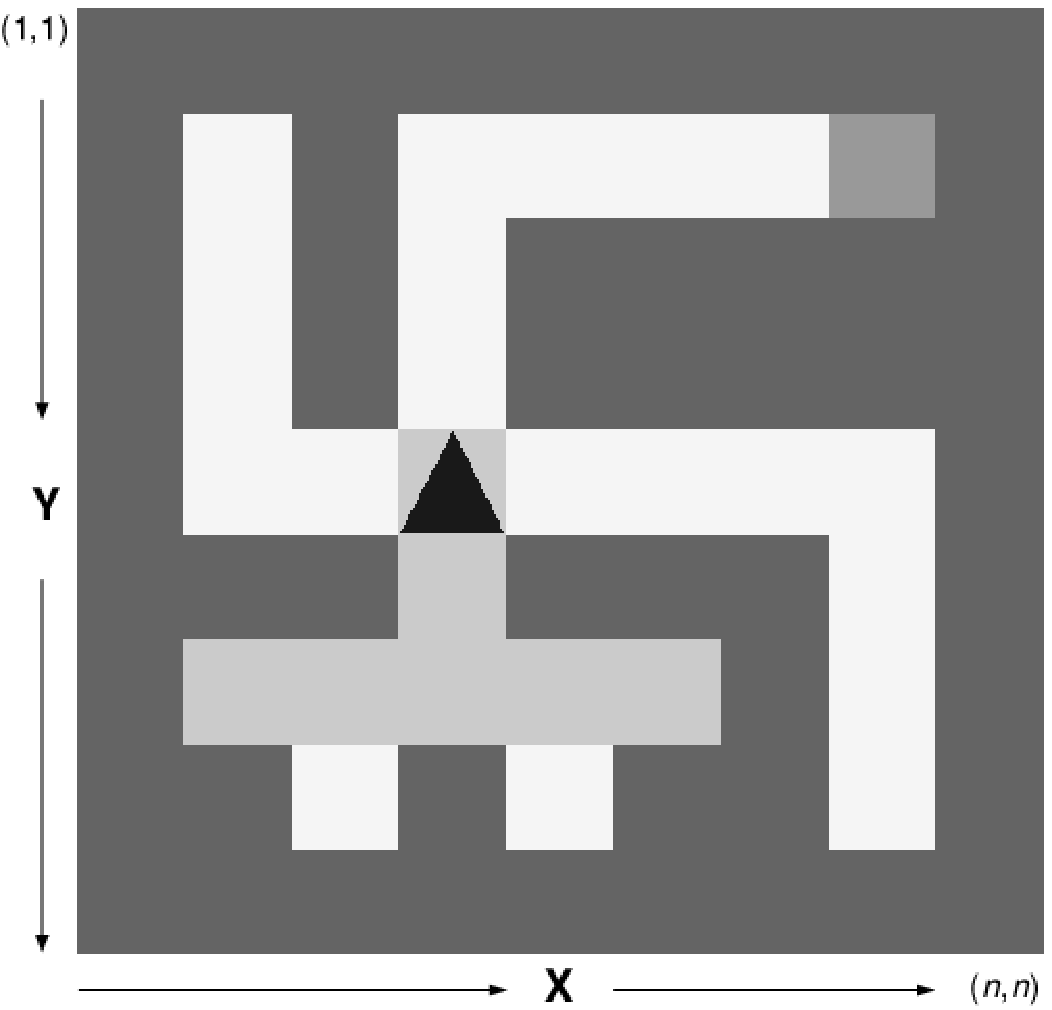
\includegraphics[width=3in]{pigs3.pdf}
\caption{The robot homing towards a target that is north-east would choose to 
go ahead (north) or right (east) as opposed to behind (south) or left (west). 
Note the relationship between the {\em x}- and {\em y}-coordinates of the robot 
and the target.
\label{northcontroller}}
\end{figure}    

\subsection{Exercise 3}

\noindent
The controller of the homing robot which we are going to 
build is based on a heading controller. \\

\noindent
Our new homing robot will choose a heading based on its current location 
and the location of the target. For instance,
if the robot is heading {\tt NORTH} and the target is to the north of it, as
in Figure~\ref{northcontroller}, then
it makes sense for the robot to select {\tt NORTH} in preference to 
{\tt SOUTH}. 
Based on this assumption, you will construct controller code to determine
whether
the target is to the {\em north}, {\em south}, {\em east} or {\em west} of 
the robot, and then 
build a heading controller that will guide 
the robot closer to the target.
Essentially what the robot is trying to do is `sense' the target and move 
towards it if at all possible. A scheme that seems inherently sensible, at 
least at the outset.

\subsubsection{Finding the target}

\noindent
It is possible to decide whether the target is to the north of the robot by 
examining the {\em y}-coordinate of the robot and the target\footnote{The 
coordinates begin (1,1) at the top left-hand corner of the maze and increase
to (n,n) at the bottom right-hand corner of the maze (the default maze is 15 by
15).}. If the robot's {\em y}-coordinate is greater than that of the target, 
then the target is north of the robot. Similarly, if the robot's 
{\em y}-coordinate is less than that of the target, then the target is to the 
south. If the {\em y}-coordinates of both the robot and target are the same, 
then you will find that both the robot and target are on the same latitude.\\

\noindent
$\diamondsuit$ Add a new method called {\tt isTargetNorth} to the file 
{\tt Broken.java}. The method should take one parameter (the robot 
itself\footnote{You will need this parameter if you are to check the 
{\em y}-coordinate of both the robot and target.}) and should return 
{\tt 1} if the target is north of the robot, {\tt -1} if the target 
is south of the robot and {\tt 0} otherwise.\\
\clearpage
\noindent
The method should look something like

\begin{verbatim}
   private byte isTargetNorth(IRobot robot) {
     byte result ...
     // returning 1 for `yes', -1 for `no' and 0 for `same latitude'
     ...
     return result;
   }
\end{verbatim}

\noindent
and should not be more than about five lines long.\\

\noindent
First sketch your solution on
paper, answering the following design questions as you go along: \\

\noindent
{\bf Design question 1:} Where in the
{\tt Broken.java} file should you locate this new method? \\

\noindent
{\bf Design question 2:} How can you determine the relative positions of 
the robot and the target? \\

\noindent
{\bf Design question 3:} What parts of the robot interface can help you 
in this calculation? \\

\noindent
Once your code compiles correctly, you should consider how to go about 
testing it. Is it possible to develop some exhaustive tests to cover all 
eventualities? You might want to look back to Section 3.3 of
{\em The Guide} to see what testing technique would me more appropriate.\\

\noindent
Consider adding some appropriate {\tt System.out.println} statements, 
and running the robot slowly to examine whether the output makes sense. 
You might find that moving the target and the robot will help you test 
more cases. Be prepared to talk about how you tested your solution and 
why you tested it in that way. \\

\noindent
$\diamondsuit$ Use your {\tt isTargetNorth} method as a basis for a second method
called {\tt isTargetEast}. This should return {\tt 1} if the target is to the 
east of the robot, {\tt -1} if the target is to the west of the target, and 
{\tt 0} otherwise.

\subsubsection{Sensing your environment}

\noindent
Currently the robot can sense its environment using the {\tt look()} function.
The function takes {\it relative} directions in order to operate correctly. The 
functions you have just written return the target's position in {\it absolute} directions 
and your controller will need to give the robot an {\it absolute} direction, so it makes
sense that you sense the environment using {\it absolute} directions. \\

\noindent
$\diamondsuit$ Write a method called {\tt lookHeading} that takes an {\it absolute} direction
and returns whether there is a {\tt WALL}, a {\tt PASSAGE} or a {\tt BEENBEFORE} square, much 
like the current {\tt look()} function. {\bf Hint:} You may need to pass the robot object to 
the function in addition to a heading.

\subsubsection{Building a heading controller}

\noindent
Using the methods that you have developed so far, it is 
possible to calculate where the target is relative to the current position of
the robot and to analyse the robots surroundings. 
As in Figure~\ref{northcontroller}, if we detect that the target
is to the north-east of the robot, it makes sense to direct it either 
north or east. That is, as long as there is not a wall in either (or both)
of these headings. \\

\noindent
$\diamondsuit$ Create a {\tt headingController} method that exhibits the following behaviour:

\begin{quote}
Given the state of the robot in the maze, the controller should {\bf return} a
heading that will head the robot towards the target if at all possible. 
This means that: ($i$) if it can select a heading that will move the robot
closer to the target then it should do so; ($ii$) it should not lead the 
robot into a wall; ($iii$) if the robot has the choice of more than one 
route, then it should randomly choose between them; ($iv$) if there
are no headings that will move the robot towards the target, pick randomly
between all available headings.
\end{quote}

\noindent
Before trying to write the software, you must have a clear understanding 
as to what this specification means exactly. \\

\noindent
{\bf Design question 1:} What should the robot controller do if travelling
{\tt NORTH} or {\tt EAST} will move the robot towards the target, and these 
passages are not blocked by walls? \\

\noindent
{\bf Design question 2:} What should the robot controller do if travelling
{\tt NORTH} or {\tt EAST} will move the robot towards the target, and there
is a wall to the north but not to the east? \\

\noindent
{\bf Design question 3:} What should the robot controller do if travelling
{\tt NORTH} or {\tt EAST} will move the robot towards the target, and there 
is a wall to the east of the robot but not to the north? \\

\noindent
Try to design your code on paper first. You might find it useful to create
a table of the scenarios that the robot might encounter and use this when 
designing your code.

\subsubsection{Testing your solution}

$\diamondsuit$ Now that the controller code is becoming more complex, it is 
important that we test it to see that it meets the desired functionality. \\

\noindent
To help with testing, we have constructed a {\em test harness} that you can
use to 
test your {\tt headingController}.  \\

\noindent
To access the test harness you need to first download it from the 
course web page; you will see that it is named {\tt ControlTest.class}
and it should be saved to the same directory as your source code. \\

\noindent
To call this test harness you need to add a couple of lines of code to 
your program. The first thing you should do is add a call to the test 
harness ({\tt ControlTest.test}) just before your robot sets its heading to the newly
chosen direction and advances, i.e.  

\begin{verbatim}
   ...
   heading = headingController(robot);
   ControlTest.test(heading, robot);
   robot.setHeading(heading);
   ...
\end{verbatim}

\noindent
This test-calling code will check each heading that your robot selects 
and compare it against a working solution. \\

\noindent
Next you need to add some code that will print the log of test results at 
the end of the robot's run. You should include the code

\begin{verbatim}
   public void reset() {
     ControlTest.printResults();
   }
\end{verbatim}

\noindent
to your class (outside the definition of the {\tt controlRobot} method,
 yet within the brackets of the whole class).\\

\noindent
These modifications will allow you to test the behaviour of your 
{\tt headingController} method. You should ensure that your robot passes 
these tests (indicated by a status report of {\bf ok}). Example test 
reports can be found on the course web page.\\

\noindent
Don't take this testing too lightly. If you were a customer buying the 
controller code then you would be pretty careful to check that it works,
particularly if you are paying good money for it.

\noindent
After thoroughly testing your solution, save it as {\tt Ex3.java}. 


\subsection{Final remarks}

\noindent
$\diamondsuit$
Can the homing robot always be expected to find the target? 
Carefully justify your answer. \\

\noindent
It is interesting that developing a smarter control algorithm does
not actually provide us with a better robot. The random robot
is preferable to the homing robot in the sense that it will eventually reach
the target, albeit after a very long wait. \\

\noindent
Also of interest is the fact that specifying and ordering a homing robot 
seemed sensible. It is quite possible that a customer, wanting a more  
sophisticated robot, would request such behaviour, unaware that the resulting 
robot would not reach the target in some cases.\\

\noindent
An answer to this sort of problem is to build a {\it prototype}. Software 
developers will often produce some small cheap code to model a potential 
solution to a coding problem. The code does not need to be shown to the 
customer, as in itself it is not important. What is important is the input and 
output behaviour that the code exhibits. A customer will be shown the 
prototype and asked to {\it inspect} the behaviour. It is at this point 
that the customer can say, `hang on, this was not what I thought it 
would do!'\\

\noindent
Prototypes are an excellent way of developing potentially expensive software.
They ensure that when a customer pays twenty million pounds for some code,
it turns out to be what they wanted.\\

\noindent
It is quite possible to write prototypes in the Java programming language,
but it is often argued that other languages are better suited to the task. For example, 
{\it functional} programming languages are favoured for the speed at which 
software can be developed and the size of the resulting code. They do not 
produce particularly fast code, but then again at the prototyping stage this 
probably does not matter. \\

\noindent
This is the end of the first coursework. Submit your work through the Tabula
submission system, making sure to include the following files:\\

\noindent
{\tt Ex1.java, Ex2.java, Ex3.java} \\

\noindent
This work will be tested on 
\deadlineone in Lab 001 of the Computer Science
building. If you have time, you might like to look through Chapters 6 and 
7 again just to make sure that you have fulfilled the requirements. Once 
you have done this you will be required to formally submit your work.